\section{Mixed Training}

For this case, adversarial examples were included in the training phase. At each epoch, the adversarial example of each images were computed, given the model at that particular epoch. Both images, clean and adversarial, were used in the training process, similar to data augmentation. This way, both the clean example and the adversarial example participate in the optimization of the parameters of the model in order to decrease the loss.

Adversarial examples are thus generated dynamically at each epoch, so that the model is trained considering its blind-spots.
The training went on for 30 epochs using 120,000 samples, half clean and half adversarial.

\begin{center}
  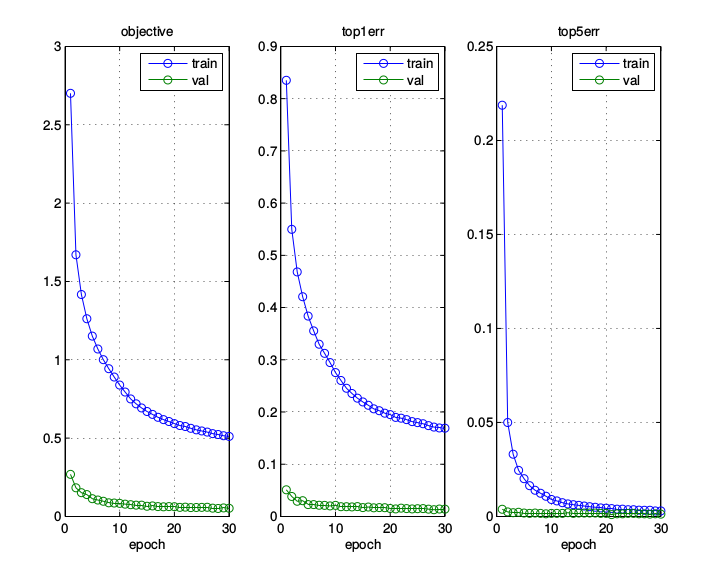
\includegraphics[width=0.7\textwidth]{img/train-mix.png}
	\label{train-mix} 
\end{center}

The tests were carried out as for the standard training.

\FloatBarrier
\begin{table}[h]
\centering
\begin{tabular}{@{}lll@{}}
\toprule
                               & Clean & Adversarial \\ \midrule
Correctly Predicted            & 98.21 & 85.28       \\
Error                          & 1.79  & 14.72       \\
Confidence                     & 97.89 & 86.30       \\
Confidence Correctly Predicted & 97.85 & 89.07       \\
Confidence Error               & 66.91 & 70.22       \\ \bottomrule
\end{tabular}
\caption{Test results for standard training model.}
\label{mixed-test}
\end{table}
\FloatBarrier

The results in Table~\ref{mixed-test} shows that for the clean samples the prediction behaved as for the standard training. For the adversarial examples, however, the results are much better than the previous case. The error rate dropped from ~97\% to ~15\% and the confidence for the misclassification also dropped significantly, from ~94\% to ~70\%, which is in a similar range as the clean samples for both cases.